%-- Intro --%

\begin{tframe}{Introduction}

This method is based on \emph{T. Carvalho}, \emph{V. Schetinger et al. }works presented in [1] and [2].
\vspace{1cm}

\textbf{Mail goal}: finding image inconsistencies based on \textbf{illuminant estimation} in order to determine if an image has been \textbf{tampered} or not.

\begin{center}
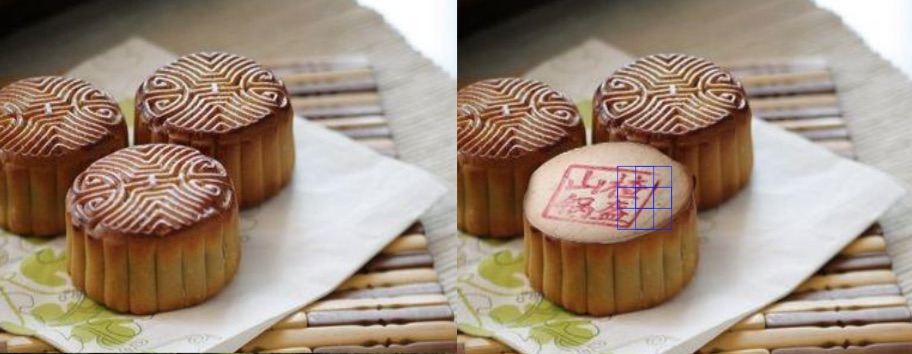
\includegraphics[width=0.6\textwidth]{images/cakes.jpg}
\end{center}

\end{tframe}

%-- Proposed method --%

\begin{tframe}{The proposed method}
\vspace{0.2cm}
The method consists on 4 steps:
\vspace{0.3cm}
\begin{enumerate}
\item \textbf{Region of Interest (ROI)} definition: manual
\vspace{0.3cm}
\item \textbf{Illuminant Map} estimation
\vspace{0.2cm}
\begin{enumerate}
\item\emph{ Generalized Greyworld Estimate} (\textbf{GGE}): statistic-based
\vspace{0.2cm}
\item \emph{Inverse-Intensity Chromaticity} (\textbf{IIC}): physics-based
\vspace{0.2cm}
\end{enumerate}
\item \textbf{Statistical difference} between the IMs
\vspace{0.2cm}
\item Image \textbf{descriptor}: based on IMs
\vspace{0.2cm}
\item \textbf{Classification} of ROIs 
\end{enumerate}

\end{tframe}

\begin{tframe}{1. Region of Interest definition}
The method proposed by Carvalho et al. [1] is restricted to images containing at least two faces. This method is able to classify as fake \textbf{any single ROIs} defined in the image.
\vspace{0.2cm}
User can \textbf{manually select} suspicious image regions.
\vspace{0.2cm}
\begin{center}
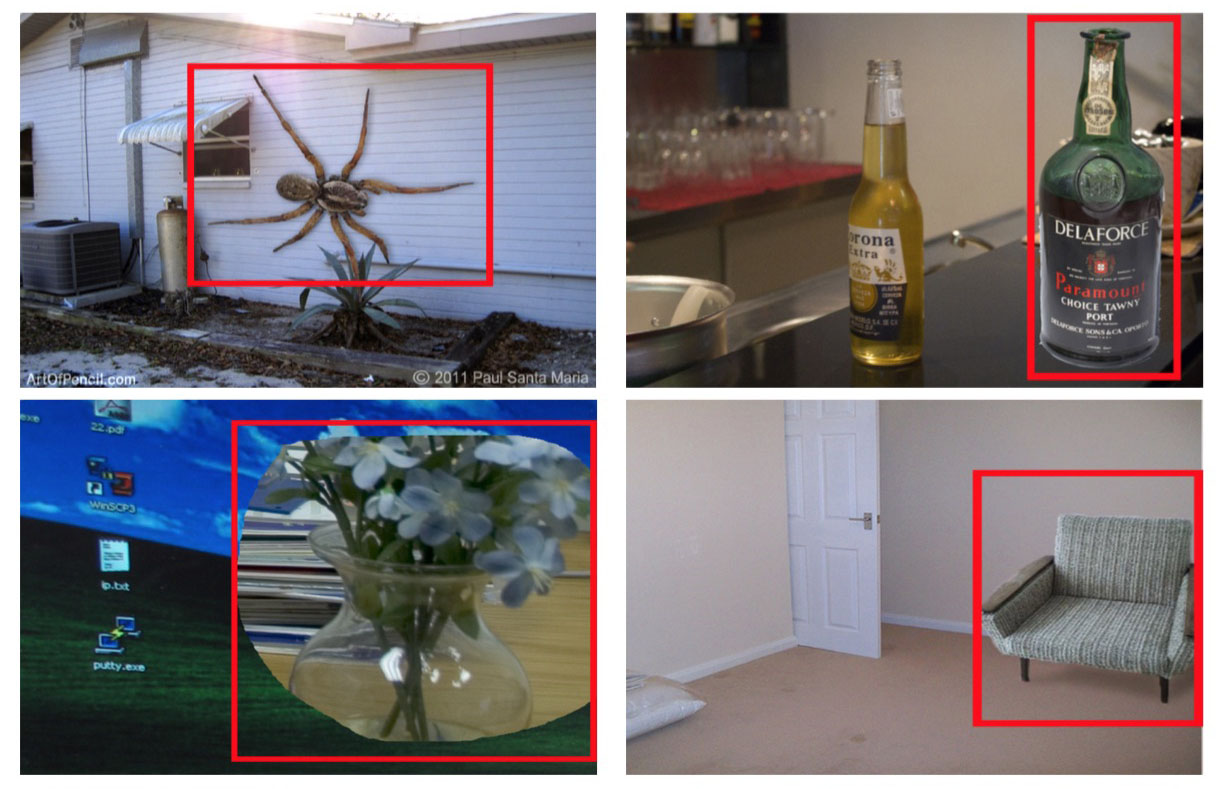
\includegraphics[width=0.6\textwidth]{images/rois.jpg}
\end{center}
\end{tframe}

\begin{tframe}{2. Illuminant Maps estimation}
\vspace{0.2cm}
For the Illuminant Maps estimation, two different techniques are used: 
\vspace{0.3cm}
\begin{enumerate}
\item A \emph{statistical-based} approach using \textbf{Generalized Grayworld Estimate (GGE)} algorithm.
\vspace{0.2cm}
\item A \emph{physics-based} approach using \textbf{Inverse-Intensity Chromaticity (IIC)} method.
\end{enumerate}

\begin{center}
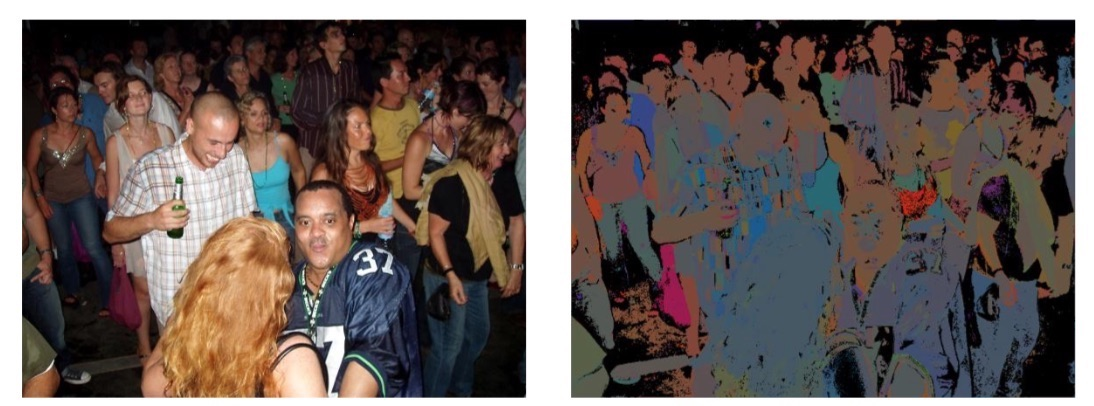
\includegraphics[width=0.7\textwidth]{images/riess.jpg}
\end{center}
\end{tframe}


\begin{tframe}{2.1 Generalized Greyworld Estimate (GGE)}
\textbf{Generalized Greyworld Estimate} is proposed in [2] as a combination of the \emph{Grey-World} and \emph{Grey-Edge method}s aimed to evaluate \textbf{color constancy}.

\vspace{0.3cm}
The main premise behind it is that in a normal well color balanced photo, the \textbf{average} of all the colors is a neutral gray. Therefore, it assumes that the \emph{Minkowski norm} of the derivative of the reflectance in a scene is \textbf{achromatic}.

\begin{equation}
k\textbf{e}^{n, p, \sigma} = (\int |\frac{\vartheta^{n}\textbf{f}^{\sigma}(\textbf{x})}{\vartheta\textbf{x}^{n}}|^{p}  d\textbf{x})^{\frac{1}{p}}
\end{equation}
\begin{footnotesize}
where $\textbf{x}$ denotes a pixel coordinate, $k$ is a scale factor, $|\cdot|$ is the absolute value operator, $\vartheta$ the partial differential operator, $\textbf{f}^{\sigma}$ is the observed intensities at position $\textbf{x}$, smoothed by a Gaussian kernel $\sigma$, $p$ is the \emph{Minkowski norm}, and $n$ is the derivative order.
\end{footnotesize}
\end{tframe}

\begin{tframe}{2.1 Generalized Greyworld Estimate (GGE)}

The illuminant estimation of (1) is a framework for low-level based illuminant estimation based on three variables:
\begin{enumerate}
\item The order $n$ of the image structure.
\item The Minkowski norm $p$ which determines the relative weights of the multiple measurements from which the final illuminant color is estimated.
\item The scale of the local measurements as denoted by $\sigma$.
\end{enumerate}
\vspace{0.2cm}
\textbf{Advantages}:
\begin{itemize}
\item the Minkowski norm of RGB values or derivatives can be computed\emph{ extremely fast}
\item the method does not require an image database taken under a \textbf{known light source}
\end{itemize}

\end{tframe}


\begin{tframe}{2.2 Inverse-Intensity Chromaticity (IIC)}
Extension of the \textbf{dichromatic reflectance model}, which states that \emph{the amount of light reflected from a point, $\textbf{x}$, of a dielectric, non-uniform material is a linear combination of diffuse reflection and specular reflection}.

\vspace{0.2cm}

Given an image taken with a \textbf{RGB camera}, the response $I_c(\textbf{x})$ for each color filter $c \in \{R, G, B\}$ is

$$
I_c(\textbf{x}) = m_d(\textbf{x})B_c(\textbf{x}) + m_s(\textbf{x})G_c(\textbf{x})
$$

\begin{small}
where $m_d$ and $m_s$ are geometric parameters of \textbf{diffuse and specular reflection}.
\vspace{0.2cm}

Let $\Delta_c(\textbf{x})$ and $\Gamma_c(\textbf{x})$ be the diffuse and \textbf{specular chromaticity}: $\Delta_c(\textbf{x}) = \frac{B_c(\textbf{x})}{\sum_{i in \{R, G, B\}} B_i(\textbf{x})}$ and $\Gamma_c(\textbf{x}) = \frac{G_c(\textbf{x})}{\sum_{i in \{R, G, B\}} G_i(\textbf{x})}$
\end{small}

\end{tframe}

\begin{tframe}{2.2 Inverse-Intensity Chromaticity (IIC)}

In this model, the intensity $I_c(\textbf{x})$ and the chromaticity $\sigma_c(\textbf{x})$ of a color channel $c \in \{R, G, B\}$ at pixel position $\textbf{x}$ are related by

\begin{equation}
\sigma_c(\textbf{x}) = p_c(\textbf{x}) \frac{1}{\sum_{i \in \{R, G, B\}} I_i(\textbf{x})} + \Gamma_c(\textbf{x})
\end{equation}
\vspace{0.2cm}

\begin{small}
where $p_c(\textbf{x}) = w_d(\textbf{x}) \sum_i B_i(\textbf{x}) (\Delta_c(\textbf{x}) - \Gamma_c(\textbf{x}))$ 
\end{small}

\begin{center}
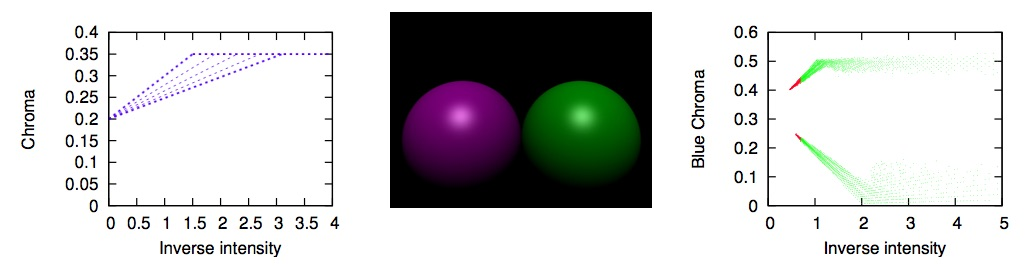
\includegraphics[width=0.6\textwidth]{images/iic.jpg}
\end{center}
The \emph{domain} of the line is determined by $\frac{1}{\sum_i I_i(\textbf{x})}$ and the \emph{range} is given by $0 \leq \sigma_c \leq 1$. Domain and range together form the \textbf{inverse-intensity chromaticity (IIC) space}.
\end{tframe}

\begin{tframe}{3. Statistical difference}
The GGE and IIC methods produce \textbf{Illuminant Maps} with different aspects for the same image.
\begin{center}
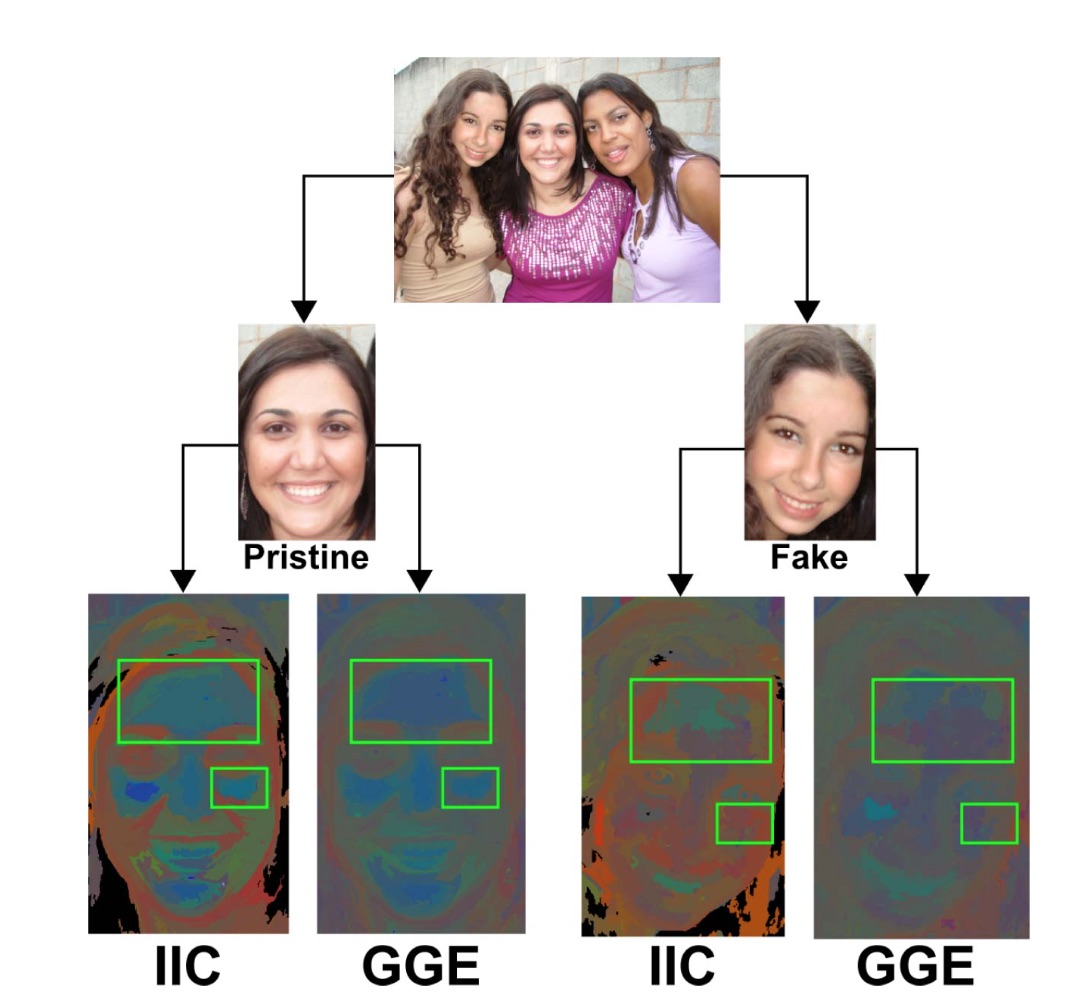
\includegraphics[width=0.6\textwidth]{images/difference.jpg}
\end{center}
\end{tframe}

\begin{tframe}{3. Statistical difference}
The appearance in terms of colors in IMs generated for \emph{pristine faces} are very similar in GGE and IIC. But, when an image contains a \textbf{fake face}, the \emph{difference} (in terms of color appearance) \emph{between GGE and IIC for this fake face is increased}.
\vspace{0.2cm}
\begin{center}
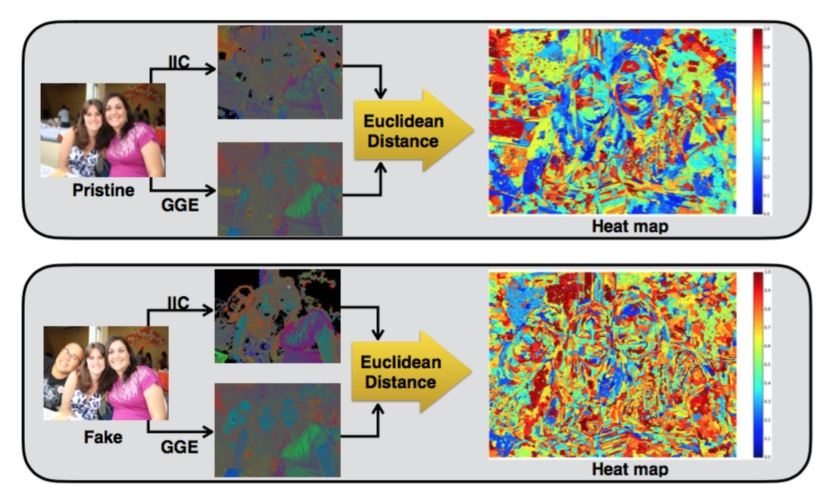
\includegraphics[width=0.6\textwidth]{images/victor.jpg}
\end{center}
\end{tframe}

\begin{tframe}{3. Statistical difference}
The heat maps highlight that \textbf{pristine images} produce a map where \textbf{shades of blue are dominants}, pointing to a \emph{lower difference between IIC and GGE maps}. \textbf{Fake images} produce a heat map where \textbf{shades of red are dominant}, indicating a \textit{more significant difference}.
\vspace{0.2cm}
\begin{center}
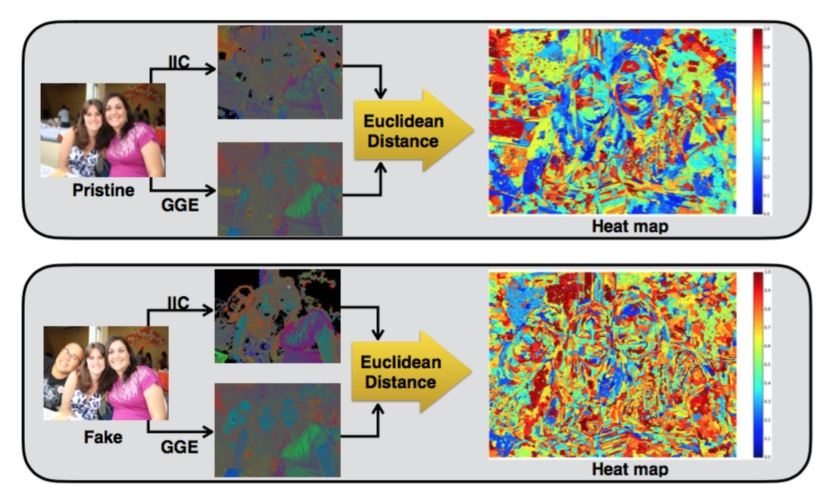
\includegraphics[width=0.6\textwidth]{images/victor.jpg}
\end{center}
\end{tframe}

\begin{tframe}{3. Statistical difference}
Given an image with $q$ \textbf{ROI} the \textbf{signature} generated by this image can be defined by
\begin{equation}
\vartheta = \frac{1}{q} \sum_{i = 1}^{q} \log (\| \lambda_n (g_{GGE})^2 - \lambda_n (f_{IIC})^2 \|)
\end{equation}
\vspace{0.2cm}
where $\lambda_n(f_{GGE})$ and $\lambda_n(f_{IIC})$ are the $n$-th higher eigenvalue extracted from the $i$-th ROI into the GGE and IIC representations.
\end{tframe}

\begin{tframe}{4. Image descriptor}
In order to \emph{eliminate the multiple ROI dependency}, a \textbf{single descriptor} combining multiple extracted eigenvalues is built:
\vspace{0.2cm}
\begin{equation}
D = \{ \mu_1, \mu_2, \ldots, \mu_{n-1},\mu_n \}
\end{equation} 
\vspace{0.2cm}
where $\mu_i$ is the difference metric based on the $i$-th higher eigenvalue extracted from one ROI.
\vspace{0.2cm}
In this way, \textbf{individual ROI }can be classified as fake or pristine.
\end{tframe}

\begin{tframe}{4. Image descriptor}
A set of difference metrics are taken into account in order to measure the difference bewtween ROIs
\vspace{0.2cm}
\begin{center}
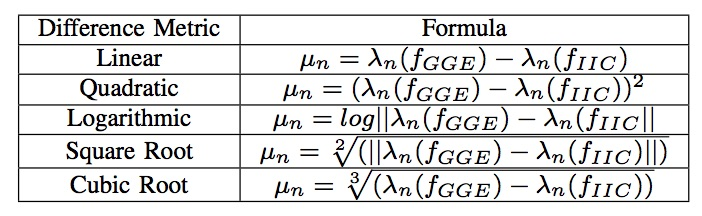
\includegraphics[width=1\textwidth]{images/metrics.jpg}
\end{center}
\end{tframe}

\begin{tframe}{5. Classification}
The classification task is performed using a \textbf{SVM classifier}. The SVM parameters are tuned with the \emph{10-fold cross-validation} techique maximizing the \textbf{accuracy} obtained in cross-validated data.

\vspace{0.2cm}

\begin{center}
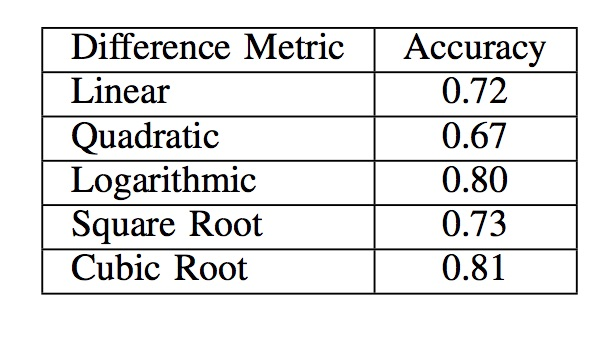
\includegraphics[width=0.6\textwidth]{images/results.jpg}
\end{center}

\end{tframe}

\begin{tframe}{Future works}
\begin{itemize}
\vspace{0.2cm}
\item \textbf{Replicate} the algorithm and perform it on a different dataset (translate code in Python/C++)
\vspace{0.2cm}
\item Use a simple \textbf{sliding window} over the whole image with different size and scale and perform the algorithm.
\vspace{0.2cm}
\item Use a \textbf{different classifier} in the classification step (\emph{KNN, NN, etc.}).
\vspace{0.2cm}
\item Exploring different \textbf{distance metrics}.
\end{itemize}
\end{tframe}



